\section{Fouriersynthese von $f(x)=x$}

Für die Fourier-Reihe der Funktion $f(x)=x$ , $-\pi < x < \pi$ berechnen sich mit $T=2\pi$ und $\omega_k = k$ nach \autoref{eq:A_k} die $A_k$ wie folgt:

\begin{align*}
  A_0 &= \frac{1}{2\pi} \int_{-\pi}^{\pi} t \symup{d}t \\
  &= 0 \\
  A_k &= \frac{1}{\pi} \int_{-\pi}^{\pi} t \cos(\omega_k t) \symup{d}t \\
  &= 0
\end{align*}

Und die Koeffizienten $B_k$ wie folgt berechnen:
\begin{align*}
  B_0 &= 0 \\
  B_k &= \frac{1}{\pi} \int_{-\pi}^{\pi} t \sin(\omega_k t) \symup{d}t \\
  &= - \frac{(-1)^k \cdot 2}{k}
\end{align*}

Damit ergeben sich folgende Koeffizienten $B_k$:

\begin{table}
  \centering
  \caption{Berechnete Koeffizienten für $f(x)=x$}
  \label{tab:b_x}
  \begin{tabular}{c c}
    \toprule 
    $k$ & $B_k$ \\ 
    \midrule 
    0 & 0.0000 \\
    1 & 2.0000 \\
    2 & -1.0000 \\
    3 & 0.6667 \\
    4 & -0.5000 \\
    5 & 0.4000 \\
    6 & -0.3333 \\
    7 & 0.2857 \\
    8 & -0.2500 \\
    9 & 0.2222 \\
    10 & -0.2000 \\
    11 & 0.1818 \\
    12 & -0.1667 \\
    13 & 0.1538 \\
    14 & -0.1429 \\
    15 & 0.1333 \\
    16 & -0.1250 \\
    17 & 0.1176 \\ 
    \bottomrule
  \end{tabular}
\end{table} 

\begin{figure}
  \centering
  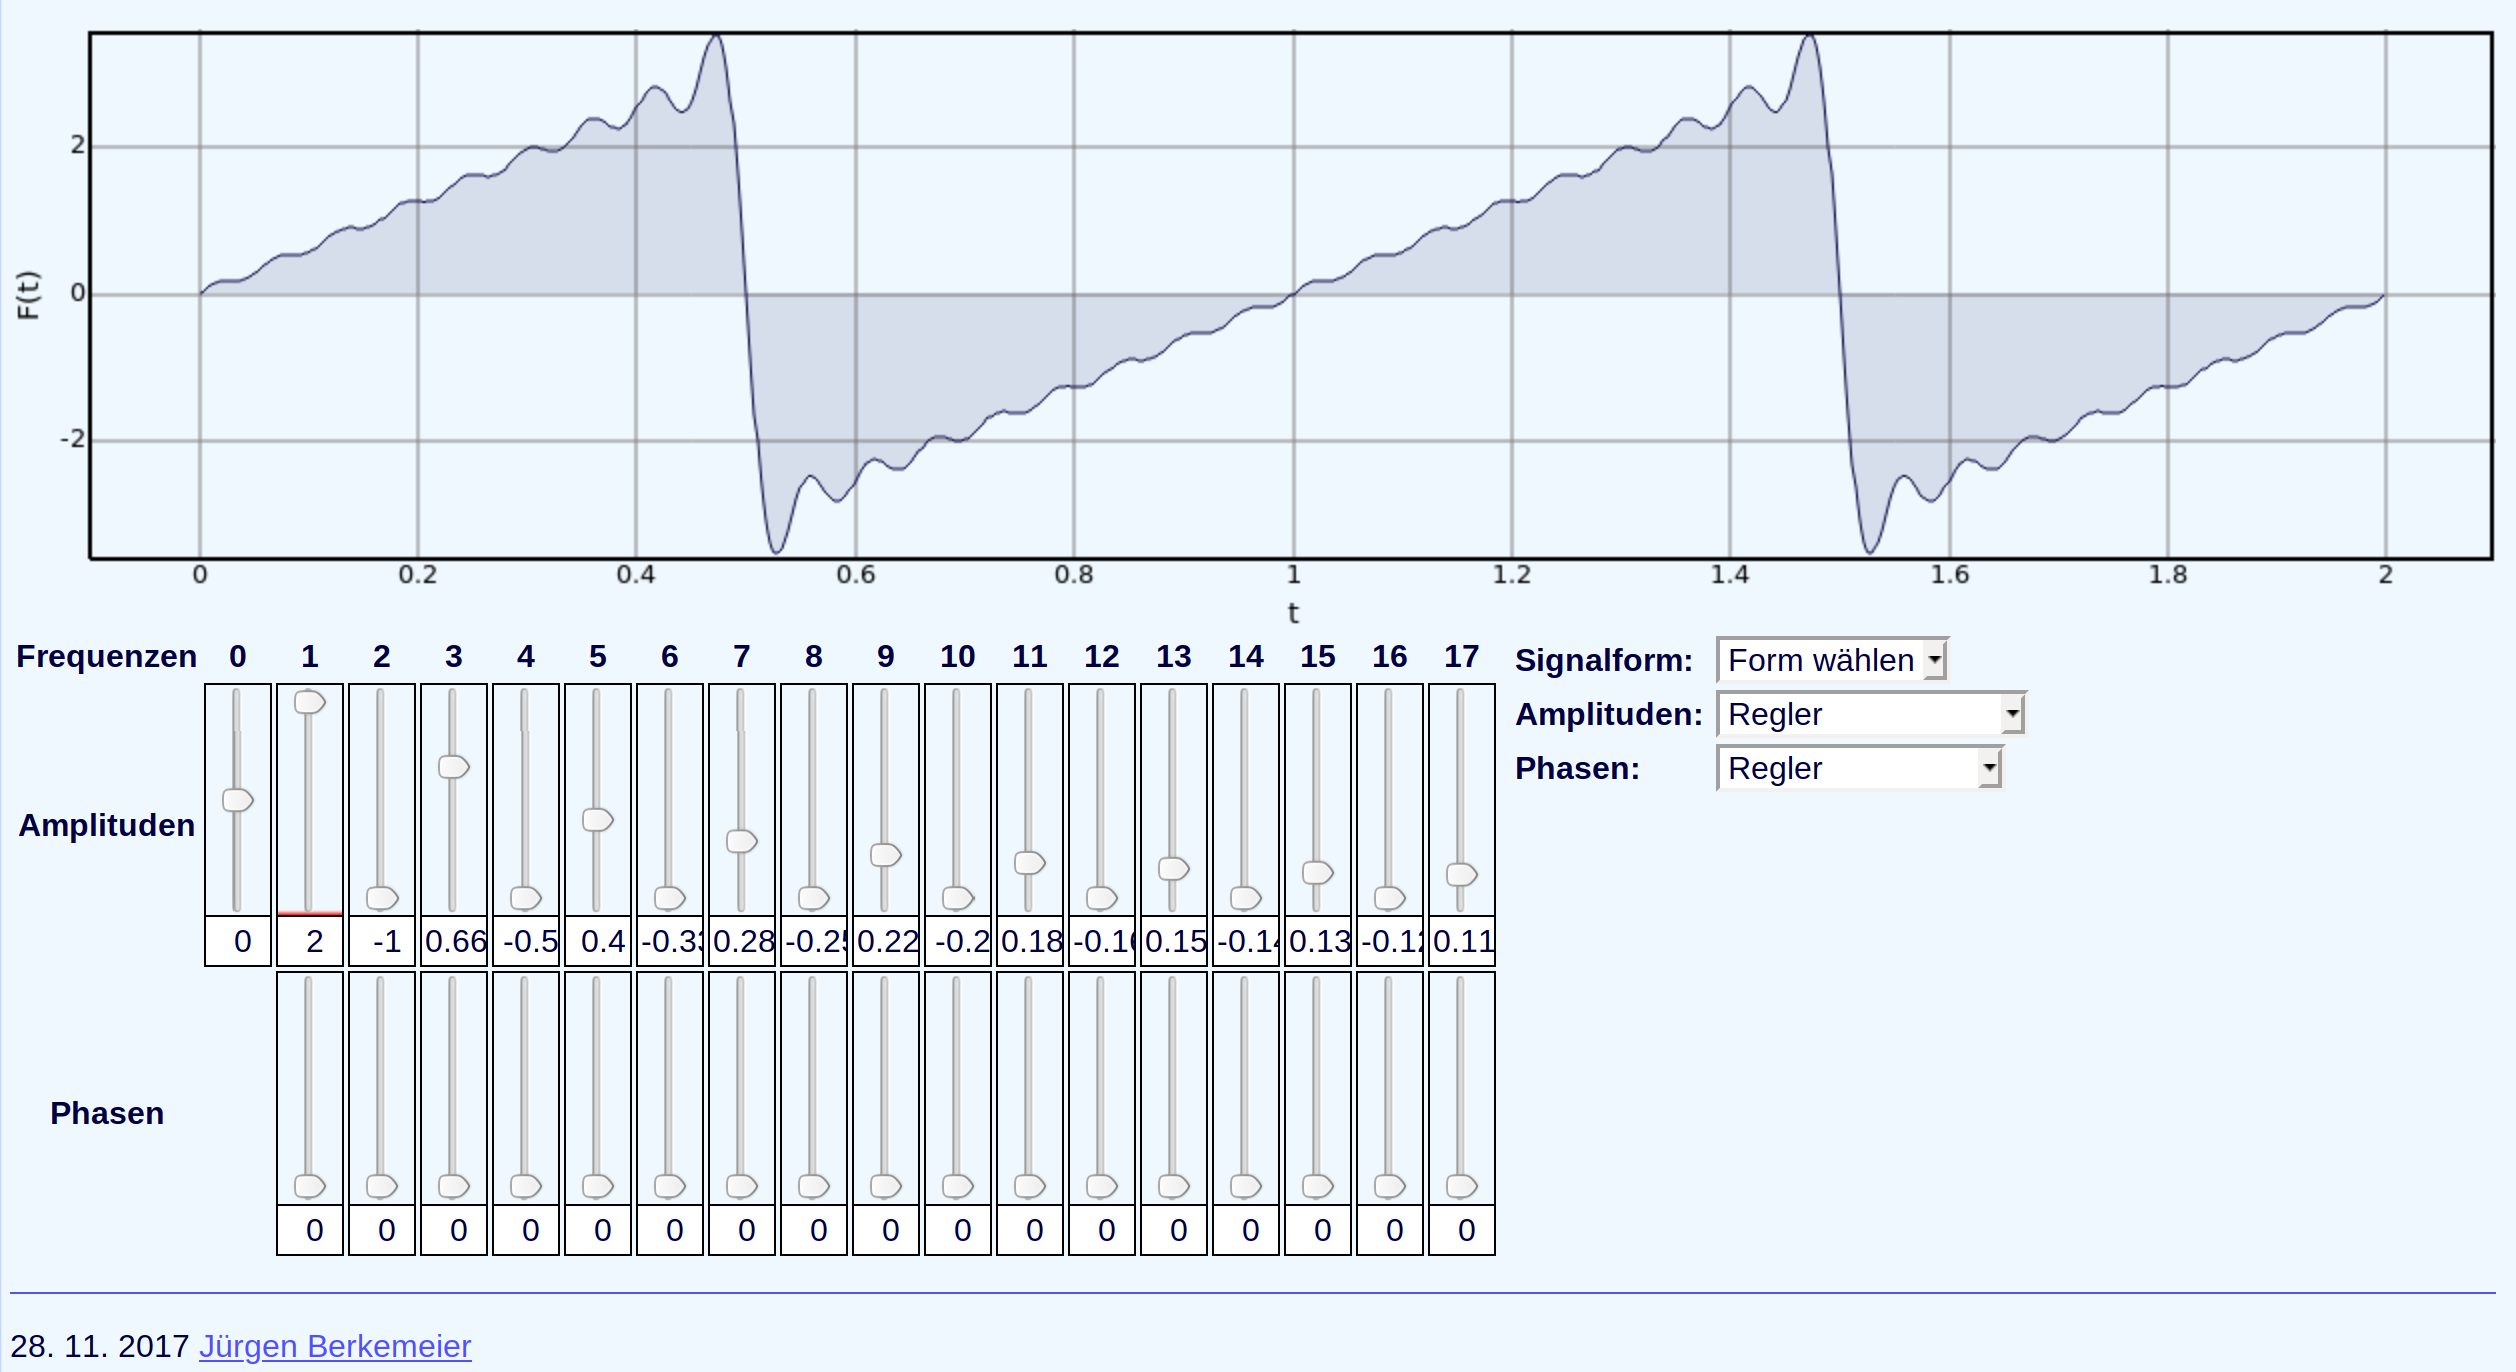
\includegraphics[width=\textwidth]{x-plot.png}
  \caption{Screenshot des Plots für die in \autoref{tab:b_x} genannte Koeffizienten von der Webseite \href{https://www.j-berkemeier.de/Fouriersynthese.html}{https://www.j-berkemeier.de/Fouriersynthese.html} wobei sich die Phase von 0° ergibt, da $A_k=0$ ist.}
\end{figure}